Die bisherigen Szenarien nutzen eine statische Kamera. Das erlaubt zwar konstante Messungen, entspricht allerdings keiner realistischen Situation. Normalerweise wird die Kamera bewegt und rotiert. Die folgenden Szenarien stellen dynamische Situationen dar, in denen die Kamera bewegt wird. In diesem Szenario wird die Kamera dauerhaft rotiert mit einer Winkelgeschwindigkeit von \SI{45}{\degree\per\second}. Eine Reihe von Screenshots, die die Rotation zeigt, ist in Abbildung~\ref{fig:rotate} zu sehen.
\begin{figure}
	\centering
	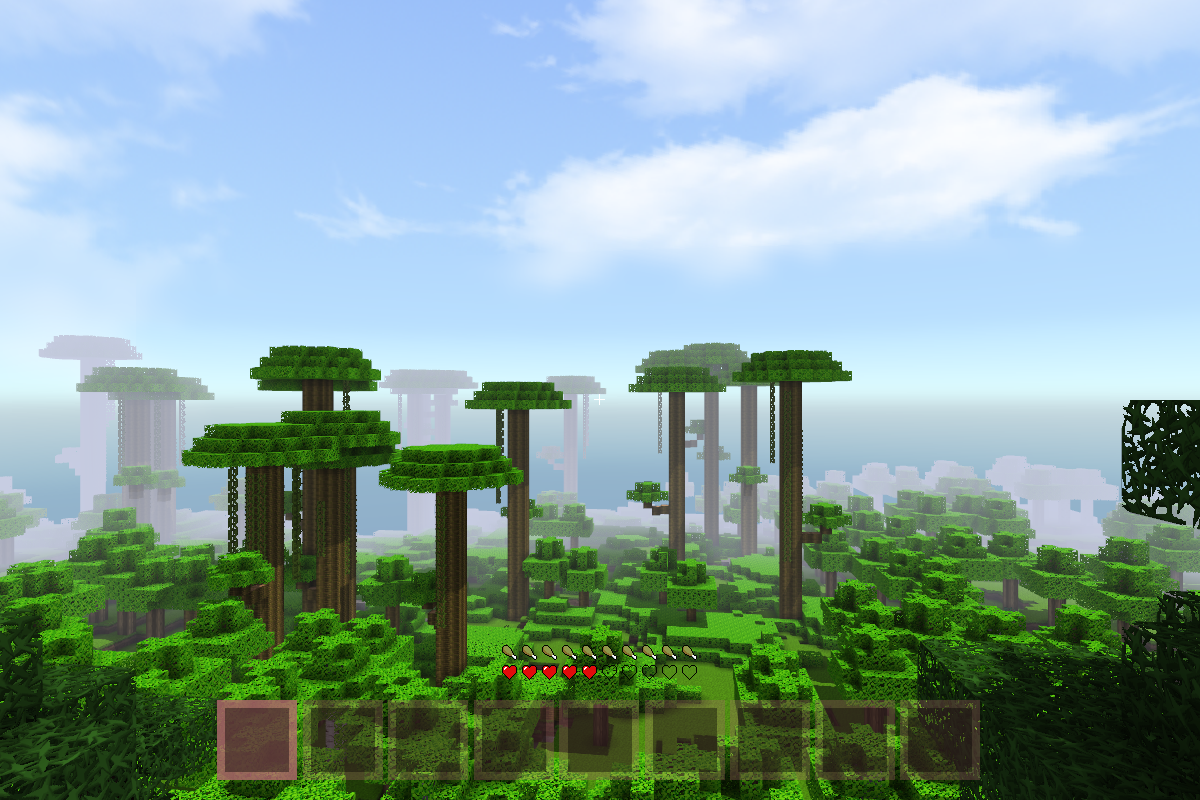
\includegraphics[width=.32\textwidth]{rotate-1.png}
	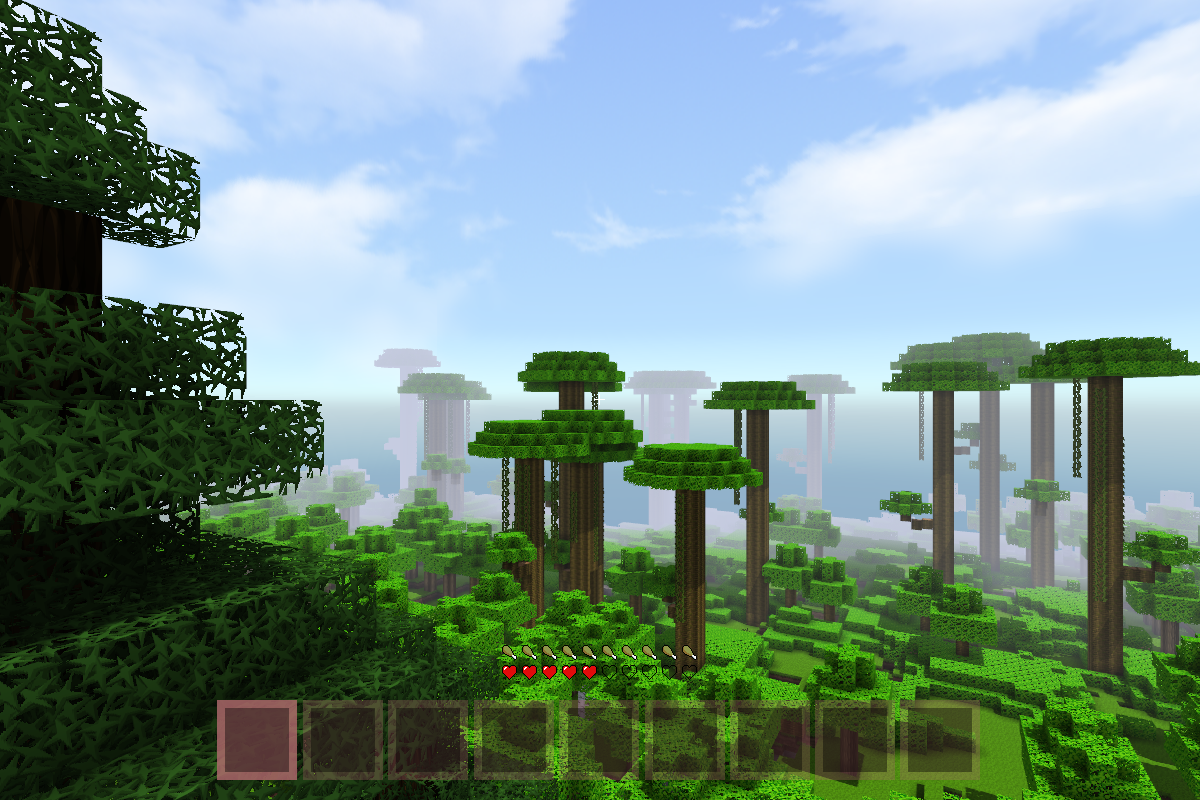
\includegraphics[width=.32\textwidth]{rotate-2.png}
	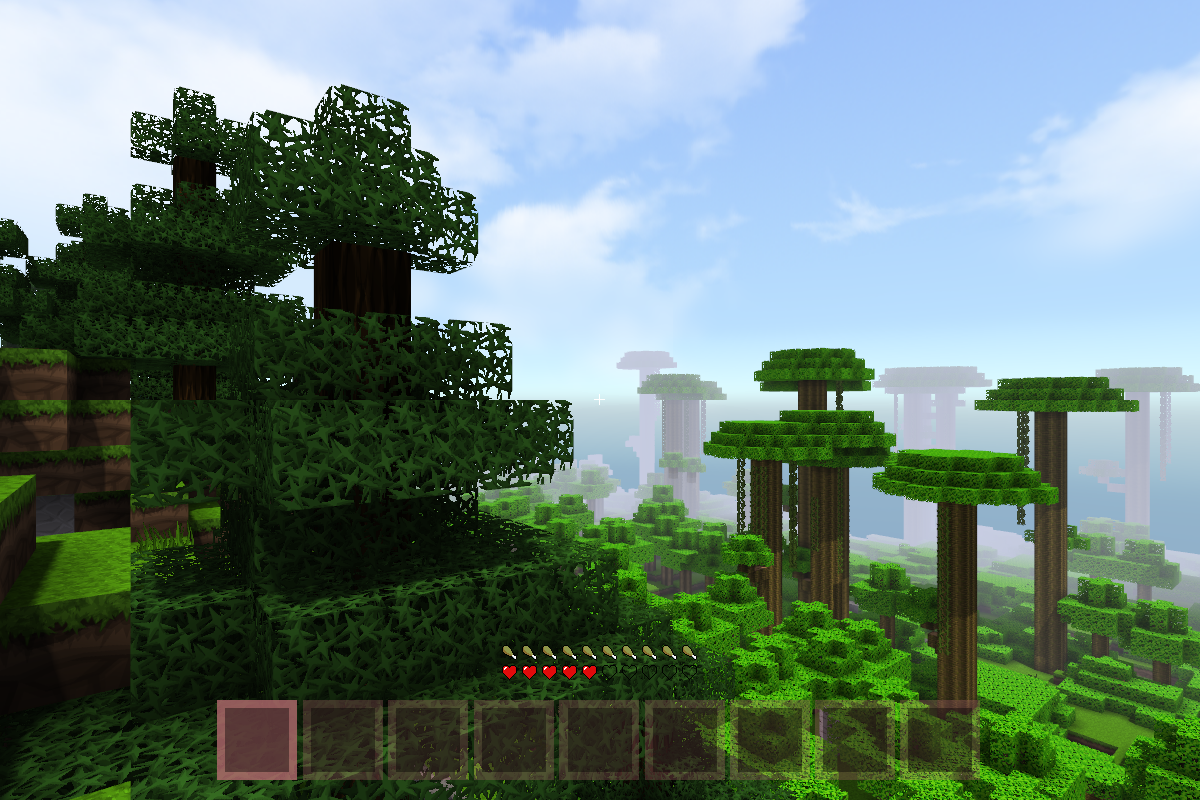
\includegraphics[width=.32\textwidth]{rotate-3.png}\\[4pt]
	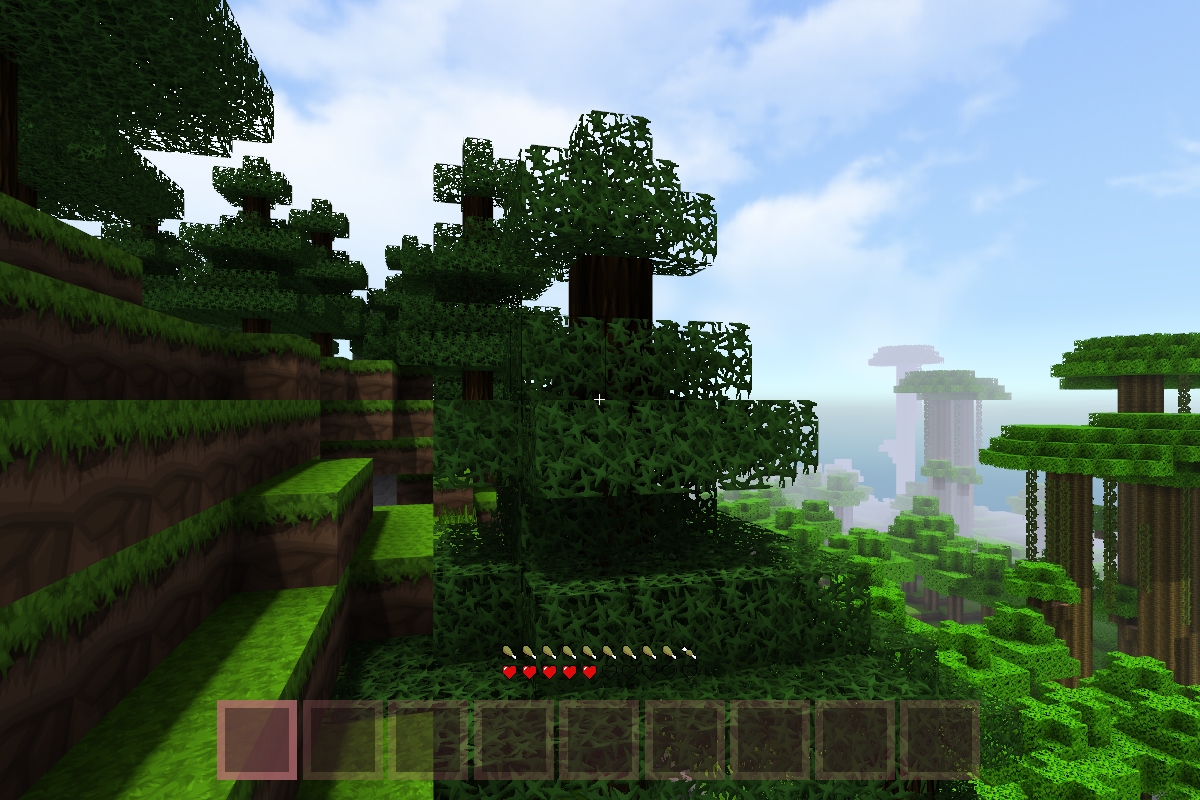
\includegraphics[width=.32\textwidth]{rotate-4.png}
	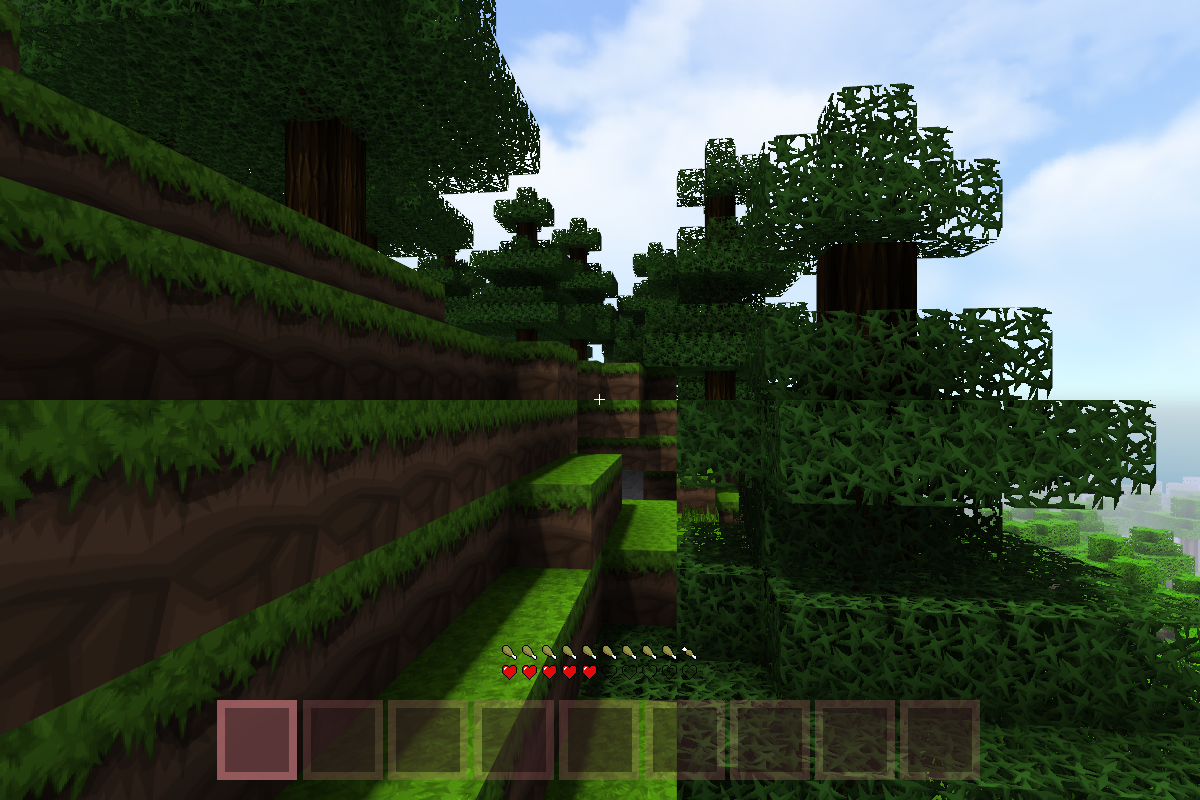
\includegraphics[width=.32\textwidth]{rotate-5.png}
	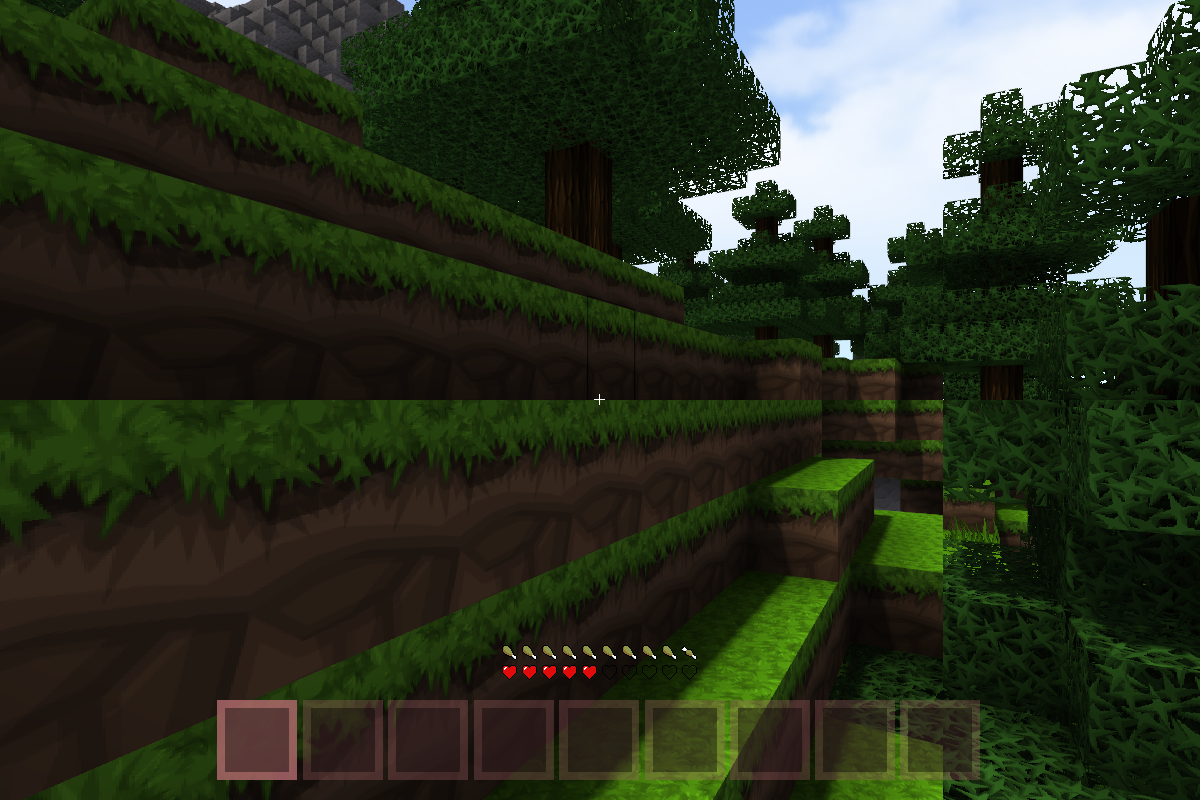
\includegraphics[width=.32\textwidth]{rotate-6.png}
	%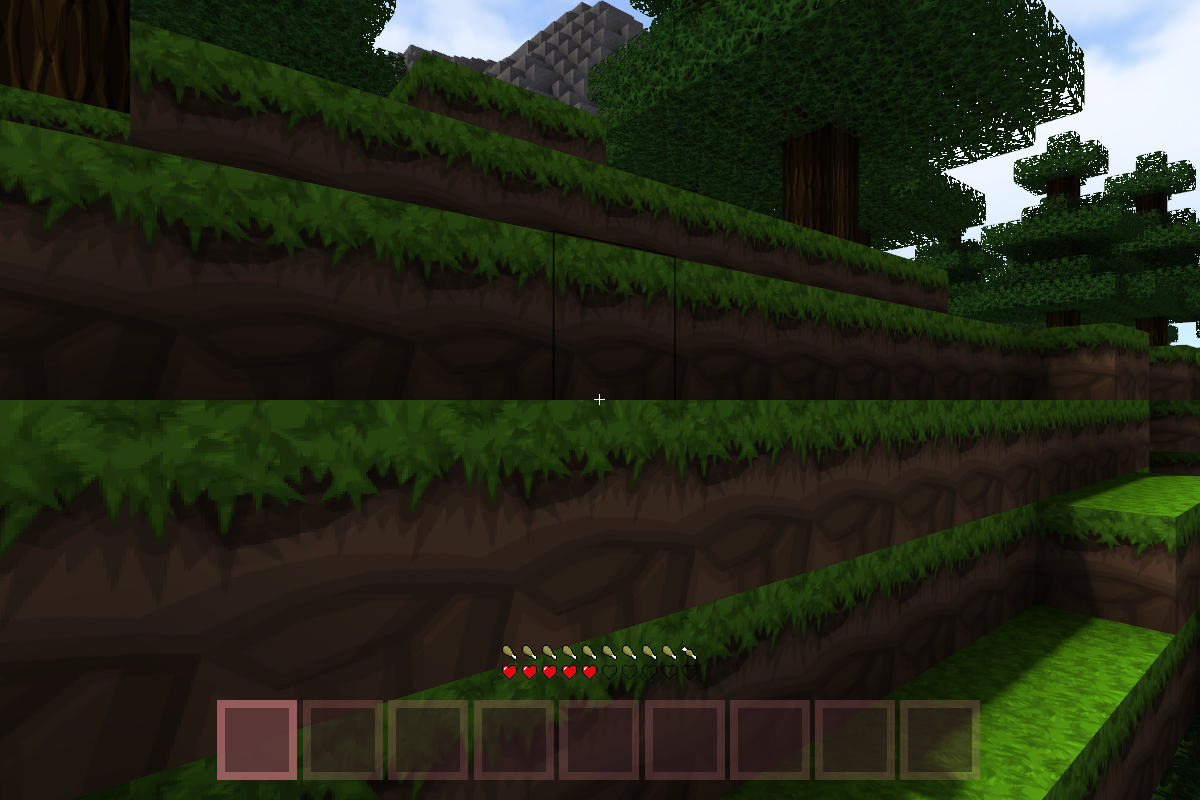
\includegraphics[width=.24\textwidth]{rotate-7.png}
	%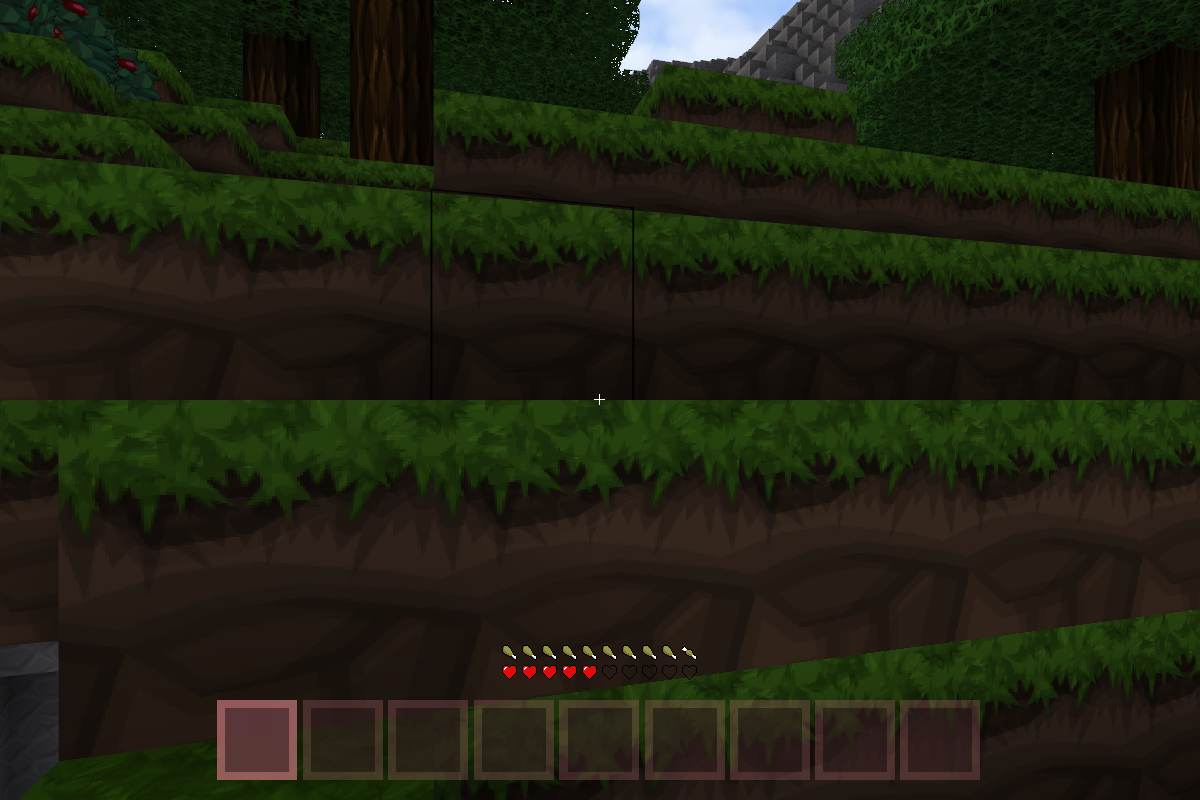
\includegraphics[width=.24\textwidth]{rotate-8.png}
	\caption{Reihe von Screenshots, die die Rotation in Szenario 4 zeigt. Die Rotationsrichtung ist gegen den Uhrzeigersinn. Die Screenshots haben einen Zeitabstand von \SI{500}{\milli\second}.}\label{fig:rotate}
\end{figure}
Wie an den Screenshots zu erkennen ist, wird auch für dieses Szenario der Seed 0 genutzt.

\paragraph{\ac{fps}}
\begin{figure}[!htbp]
	\fpsplot{seed-0-rotate}
	\caption{Seed 0 Rotation}\label{fig:seed-0-rotate-fps}
\end{figure}

\paragraph{\ac{cpu}}
\begin{figure}[!htbp]
	\cpuplot{seed-0-rotate}
	\caption{Seed 0 Rotation}\label{fig:seed-0-rotate-cpu}
\end{figure}

\paragraph{\ac{gpu}}
\begin{figure}[!htbp]
	\gpuplot{seed-0-rotate}
	\caption{Seed 0 Rotation}\label{fig:seed-0-rotate-gpu}
\end{figure}

\paragraph{\ac{ram}}
\begin{figure}[!htbp]
	\memplot{seed-0-rotate-single-mem.csv}
	\memplot{seed-0-rotate-multi-mem.csv}
	\caption{Seed 0 Rotation}\label{fig:seed-0-rotate-mem}	
\end{figure} 

